% !TeX encoding = ISO-8859-1
%----------------------------------------------------------------------------------------
%	Packages and others definitions
%----------------------------------------------------------------------------------------
\usepackage[T1]{fontenc}
\usepackage[latin1]{inputenc}
\usepackage[french]{babel}
\usepackage{lmodern}
\usepackage{amsmath}
\usepackage{minitoc}
\setcounter{minitocdepth}{1}
\usepackage{classicthesis} 
\usepackage[top=2cm,bottom=3cm,left=2cm,right=2cm,headsep=10pt,a4paper]{geometry}
%--------------------------------------------------------------------------------
%  Package que moi meme j'ai ajoute
%---------------------------------------------------------------------------------
\usepackage{multirow}
\usepackage{longtable}
\usepackage{multicol}
\usepackage{float}
\DeclareUnicodeCharacter{2212}{-}
\DeclareUnicodeCharacter{2217}{-}
\usepackage{graphicx}
\graphicspath{{Pictures/}}

\usepackage{tikz}
\usepackage{charter}

\usepackage{xcolor}
\definecolor{lightGreen}{RGB}{0,102,0}
\definecolor{lightBlue}{RGB}{179,0,0}
\definecolor{lightPurple}{RGB}{91,155,213}

%\usepackage{titletoc}
\usepackage{url}
%\usepackage{ifthen}\usepackage[style=alphabetic,citestyle=numeric,sorting=nyt,sortcites=true,autopunct=true,babel=hyphen,hyperref=true,abbreviate=false,backref=true,backend=biber]{biblatex}
%\addbibresource{Bibliography.bib} % BibTeX bibliography file
%\defbibheading{bibempty}{}

\usepackage{calc} % For simpler calculation - used for spacing the index letter headings correctly
\usepackage{makeidx} % Required to make an index
\makeindex % Tells LaTeX to create the files required for indexing

\usepackage{fancyhdr}

\usepackage{listings}
\lstset{
    captionpos=t,
    basicstyle={\ttfamily\footnotesize},
    numbers=left,
    numberstyle={\ttfamily\Huge},
    tabsize=2,
    language=Java,
    float,
    frame=single,
}

\usepackage{algorithmicx}
\usepackage{hhline}
\usepackage[ruled]{algorithm}
\usepackage{algcompatible}
\usepackage{algpseudocode}
\usepackage{algpascal}
\usepackage{algc}
\makeatletter
\renewcommand{\ALG@name}{Algorithme}
\renewcommand{\listalgorithmname}{Liste des \ALG@name s}
\makeatother
\newcommand{\packFrench}{
\algrenewcommand\algorithmicwhile{\textbf{tant que}}
\algrenewcommand\algorithmicif{\textbf{si}}
\algrenewcommand\algorithmicthen{\textbf{alors}}
\algrenewcommand\algorithmicelse{\textbf{sinon}}
\algrenewcommand\algorithmicfor{\textbf{pour}}
%\algrenewcommand\algorithmicto{\textbf{à}}
\algrenewcommand\algorithmicdo{\textbf{faire}}
\algrenewcommand\algorithmicend{\textbf{fin}}
\algrenewcommand\algorithmicreturn{\textbf{retourn�}}
}

%----------------------------------------------------------------------------------------
%	HYPERLINKS IN THE DOCUMENTS
%----------------------------------------------------------------------------------------

\usepackage{hyperref}
\hypersetup{hidelinks,backref=true,pagebackref=true,hyperindex=true,colorlinks=false,breaklinks=true,urlcolor= lightGreen,bookmarks=true,bookmarksopen=false,pdftitle={Title},pdfauthor={Author}}
\usepackage{bookmark}
\bookmarksetup{
open,
numbered,
addtohook={%
\ifnum\bookmarkget{level}=0 % chapter	
\bookmarksetup{bold}%
\fi
\ifnum\bookmarkget{level}=-1 % part
\bookmarksetup{color=lightGreen,bold}%
\fi
}
}

%----------------------------------------------------------------------------------------
%	FLOATS: TABLES, FIGURES AND CAPTIONS SETUP
%----------------------------------------------------------------------------------------

\usepackage{tabularx} % Better tables
\usepackage{multirow}
\setlength{\extrarowheight}{3pt} % Increase table row height
\newcommand{\tableheadline}[1]{\multicolumn{1}{c}{\spacedlowsmallcaps{#1}}}
\newcommand{\myfloatalign}{\centering} % To be used with each float for alignment
\usepackage{caption}
\captionsetup{font=small}
\usepackage{subfig}
\usepackage{makecell}
\usepackage{ragged2e}
\usepackage{array}

\usepackage{mathtools}
\DeclarePairedDelimiter\ceil{\lceil}{\rceil}
\DeclarePairedDelimiter\floor{\lfloor}{\rfloor}
%-------------------------------------------------------------------------------------
%	COVER PAGE MAKING
%-------------------------------------------------------------------------------------

%----------------------------------------------------------------------------------------
%	HEADER THEME
%----------------------------------------------------------------------------------------

%%----------------------------------------------------------------------------------------
%%	TITLE THEME
%%----------------------------------------------------------------------------------------
%\newcommand*{\rotrt}[1]{\rotatebox{90}{#1}} % Command to rotate right 90 degrees
%\newcommand*{\rotlft}[1]{\rotatebox{-90}{#1}} % Command to rotate left 90 degrees
%
%\newcommand*{\titleBC}{\begingroup % Create the command for including the title page in the document
%\centering % Center all text
%
%\def\CP{\textit{\Huge THEME}} % Title
%
%\settowidth{\unitlength}{Set the width of the curly brackets to the width of the title ...................................}
%{\color{lightBlue}\resizebox*{\unitlength}{\baselineskip}{\rotrt{$\}$}}} \\[\baselineskip] % Print top curly bracket
%\textcolor{lightPurple}{\CP} \\[\baselineskip] % Print title
%{\color{lightGreen}\Large A COARSE-GRAINED PARALLEL ALGORITHM \\[0.5\baselineskip] FOR THE MATRIX CHAIN ORDER PROBLEM} \\ % Tagline or further description
%{\color{lightBlue}\resizebox*{\unitlength}{\baselineskip}{\rotlft{$\}$}}} % Print bottom curly 
%
%\endgroup}

%----------------------------------------------------------------------------------------
%	TITLE PAGE
%----------------------------------------------------------------------------------------
%\newcommand*{\titleBC}{\begingroup % Create the command for including the title page in the document
%\centering % Center all text
%
%\textcolor{lightBlue}{\rule{\textwidth}{1.6pt}}\vspace*{-\baselineskip}\vspace*{2pt} % Thick horizontal line
%\textcolor{lightBlue}{\rule{\textwidth}{0.4pt}}\\[\baselineskip] % Thin horizontal line
%{\large {\textcolor{lightGreen}{\textsc{UNE APPROCHE HYBRIDE DE R�SOLUTION DU PROBL�ME \\[0.5\baselineskip] D'ALLOCATION DE FR�QUENCES: } \\[0.5\baselineskip] applications dans les r�seaux sans fil}}}\\[\baselineskip] % Title
%
%\textcolor{lightBlue}{\rule{\textwidth}{0.4pt}}\vspace*{-\baselineskip}\vspace{3.2pt} % Thin horizontal line
%\textcolor{lightBlue}{\rule{\textwidth}{1.6pt}}\\[\baselineskip] % Thick horizontal line
%
%\endgroup}

%----------------------------------------------------------------------------------------
%	TITLE PAGE
%----------------------------------------------------------------------------------------
\newcommand*{\rotrt}[1]{\rotatebox{90}{#1}} % Command to rotate right 90 degrees
\newcommand*{\rotlft}[1]{\rotatebox{-90}{#1}} % Command to rotate left 90 degrees
\newcommand*{\titleBC}{\begingroup % Create the command for including the title page in the document
\centering % Center all text

\settowidth{\unitlength}{Set the width of the curly brackets to the width of the title ...................................}
~\\[\baselineskip]~\\[\baselineskip]
\textcolor{lightBlue}{\resizebox*{\unitlength}{\baselineskip}{\rotrt{$\}$}}}\\[0.5\baselineskip] % Thin horizontal line
{\large{\textcolor{lightBlue}{\textsc{ APPROCHE D'INTELLIGENCE ARTIFICIELLE POUR \\[0.5\baselineskip] L'�VALUATION DE LA QUALIT� DU LOGICIEL }}}} % Title
\textcolor{lightBlue}{\resizebox*{\unitlength}{\baselineskip}{\rotlft{$\}$}}}

\endgroup}

%----------------------------------------------------------------------------------------
%	MAKE TILE PAGE
%----------------------------------------------------------------------------------------

\newcommand*{\makeCoverPage}{\begingroup
\thispagestyle{empty}
\begin{tikzpicture}[remember picture,overlay]
\coordinate [below=1cm] (midpoint) at (current page.north);
\node at (current page.north west)
{\begin{tikzpicture}[remember picture,overlay]
\node[anchor=north west,inner sep=0pt] at (0,0) {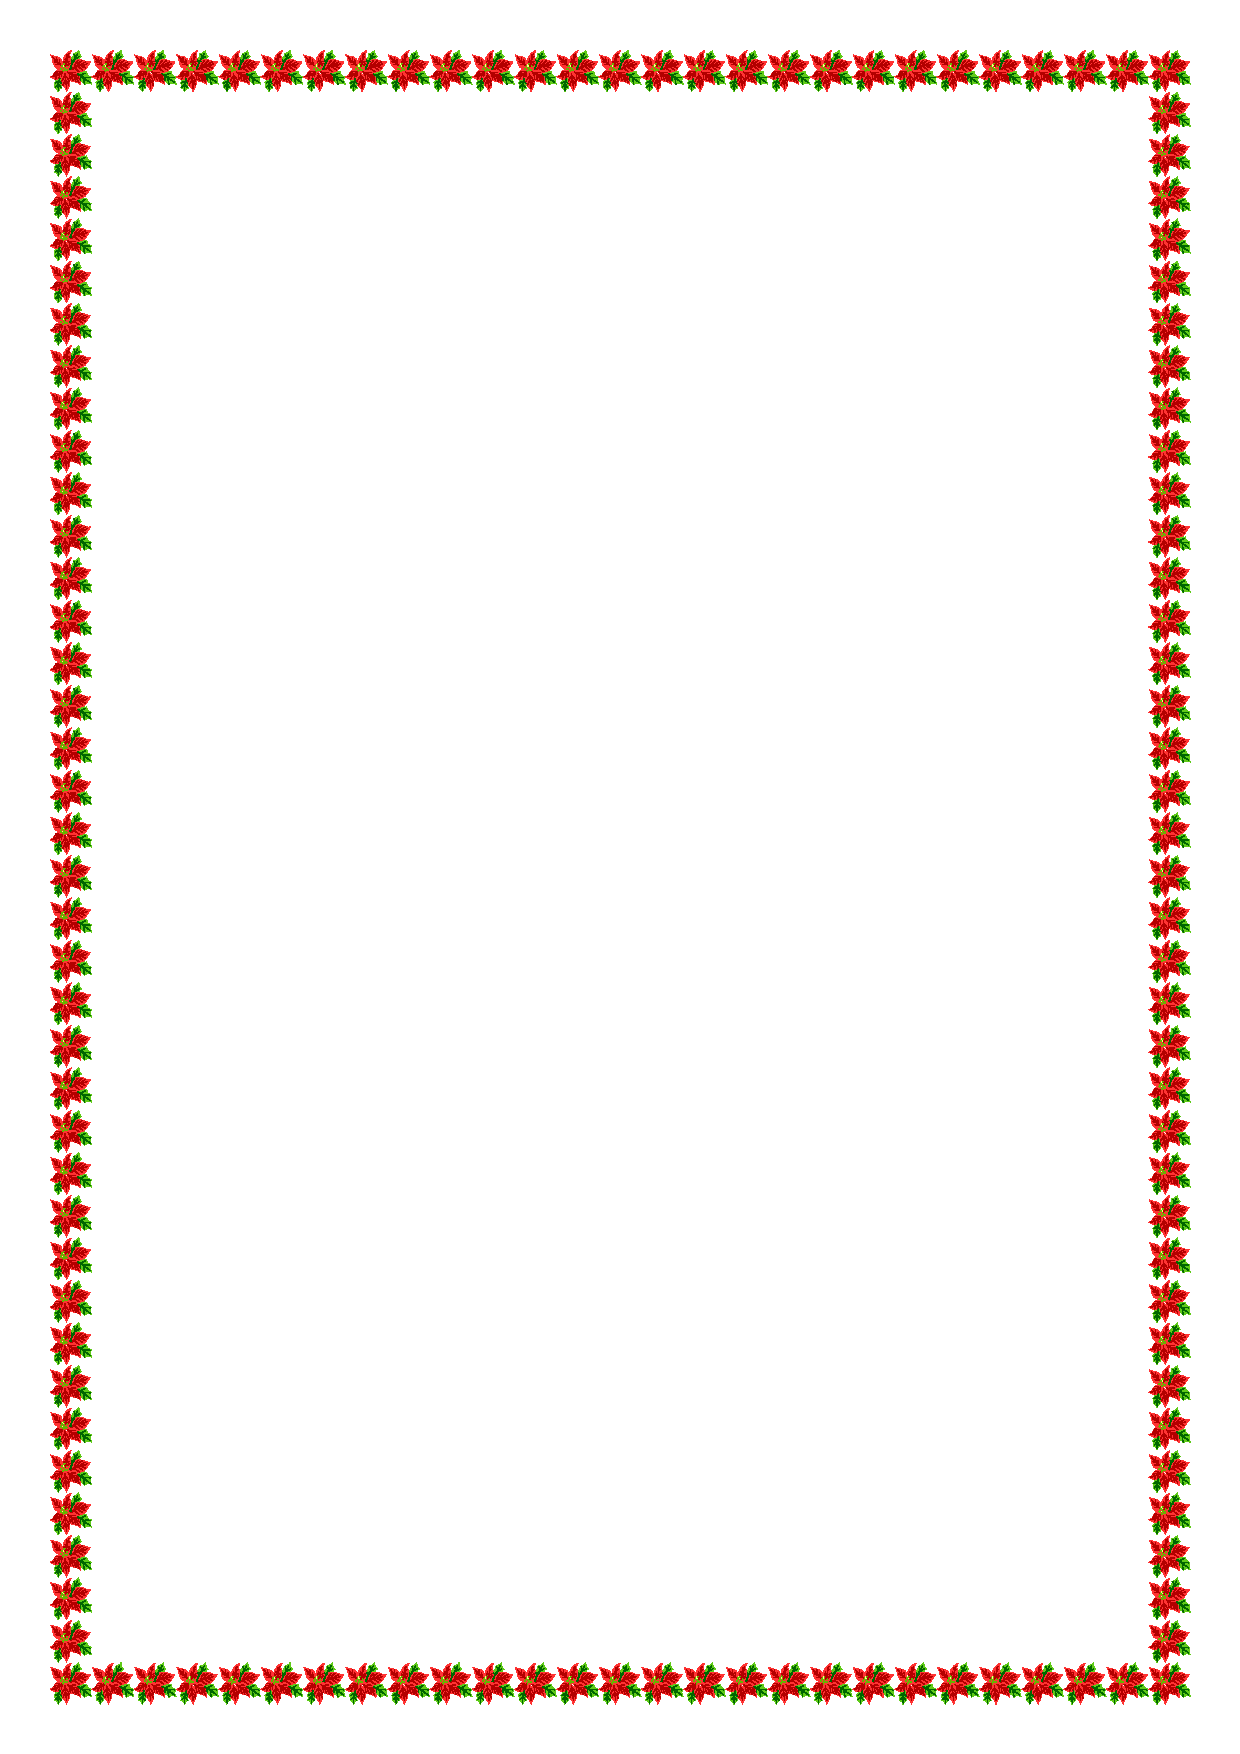
\includegraphics[width=\paperwidth]{background.pdf}}; % Background image
\draw[anchor=north] (midpoint) node [fill=white,fill opacity=0,text opacity=1,inner sep=1cm]{
\hspace{1.3cm}\parbox[b]{0.5\textwidth}{
\centering
\textsc{\textbf{\MakeTextUppercase R\'EPUBLIQUE DU CAMEROUN}}\\
\textsc{\textbf{\MakeTextUppercase PAIX-TRAVAIL-PATRIE}}\\
\textsc{\textbf{*********}} \\
\textsc{\textbf{\MakeTextUppercase UNIVERSIT\'E DE DSCHANG}}\\
\textsc{\textbf{*********}} \\
\textsc{\textbf{\'ECOLE DOCTORALE}} \\

\vfill
}

\parbox[c]{0.1\textwidth}{
\hfill 
\includegraphics[scale=0.7]{imgUDS.png} \hfill
}

\parbox[b]{0.5\textwidth}{
\centering
\textsc{\textbf{\MakeTextUppercase REPUBLIC OF CAMEROON}}\\
\textsc{\textbf{\MakeTextUppercase PEACE-WORK-FATHERLAND}}\\
\textsc{\textbf{*********}} \\
\textbf{\scshape\MakeTextUppercase UNIVERSITY OF DSCHANG}\\
\textsc{\textbf{*********}} \\
\textsc{\textbf{POSTGRADUATE SCHOOL}} \\

\vfill
}
\hspace{1.7cm}
};
\end{tikzpicture}};


\coordinate [below=6cm] (midpoint) at (current page.north);
\node at (current page.north west)
{\begin{tikzpicture}[remember picture,overlay]
\draw[anchor=north] (midpoint) node [fill=white,fill opacity=0,text opacity=1,inner sep=1cm]{
\parbox{\paperwidth}{
	\centering
	\textsc{\large\textbf{DSCHANG SCHOOL OF SCIENCES AND TECHNOLOGY}}\\
	\vspace{0.8cm}
	%\textsc{\textbf{D\'EPARTEMENT DE MATH\'EMATIQUES-INFORMATIQUE}}\\
	%\textsc{\textbf{\textit{DEPARTMENT OF MATHEMATICS AND COMPUTER SCIENCE}}}\\
	%\vspace{0.8cm}
	%{\scshape \textbf{LABORATOIRE D'INFORMATIQUE FONDAMENTALE APPLIQU\'EE} (\textit{LIFA})}
	{\large\textbf{Unit\'e de Recherche d'Informatique Fondamentale,\\ Ing\'enierie et Appliqu\'ee} (\textit{URIFIA})}\\\vspace{0.4cm}
	{\large\scshape\textbf{SUJET:}}\\
	\vfill
	
}
};
\end{tikzpicture}};


\coordinate [below=9cm] (midpoint) at (current page.north);
\node at (current page.north west)
{\begin{tikzpicture}[remember picture,overlay]
\draw[anchor=north] (midpoint) node [fill=white,fill opacity=0,text opacity=1,inner sep=1cm]{
\parbox{\paperwidth}{
\titleBC
}
};
\end{tikzpicture}};


\coordinate [below=19cm] (midpoint) at (current page.north);
\node at (current page.north west)
{\begin{tikzpicture}[remember picture,overlay]
\draw[anchor=north] (midpoint) node [fill=white,fill opacity=0,text opacity=1,inner sep=1cm]{
\parbox[t][2cm][c]{\textwidth}{
\centering
\vfill
%{\Large\scshape\MakeTextUppercase M�moire} \\[0.5\baselineskip]

M�moire soutenu publiquement en vue de l'obtention du dipl�me de\\ \textbf{Master en Informatique} \\[0.5\baselineskip]
{\Large\scshape\MakeTextUppercase Option : \textcolor{lightBlue}{informatique fondamentale}} \\[0.5\baselineskip]

{\Large\scshape\MakeTextUppercase Sp�cialit� : \textcolor{lightBlue}{r�seaux et services distribu�s}} \\[\baselineskip]
{\Large\scshape\MakeTextUppercase par:} \\[0.5\baselineskip]

{\Large\scshape\MakeTextUppercase NKEUGA NGUELIEKAM Stephane}\\

{\scshape\MakeTextUppercase matricule : CM-UDS-$18$SCI$3207$} \\

{\textit{Licence en Informatique}}

\vspace{4cm}
}
};
\end{tikzpicture}};


\coordinate [below=22.5cm] (midpoint) at (current page.north);
\node at (current page.north west)
{\begin{tikzpicture}[remember picture,overlay]
\draw[anchor=north] (midpoint) node [fill=white,fill opacity=0,text opacity=1,inner sep=1cm]{
%\parbox[b][4cm][t]{8cm}{
%\flushleft
%\vfill
%{\scshape\MakeTextUppercase Sous l'encadrement acad�mique de :} \\[0.5\baselineskip]
%
%{\scshape\MakeTextUppercase Dr Kengne Tchendji Vianney} \\[0.5\baselineskip]
%
%{(Charg� de cours, Universit� de Dschang)} %\color{white}
%
%}
%
%\parbox[b][4cm][t]{8cm}{
%\flushright
%\vfill
%{\scshape\MakeTextUppercase Ann�e acad�mique:} \\[0.5\baselineskip]
%%{\color{white} quelque chose!} : petite astuce pour cacher le texte afin d'avoir une bonne mise en forme
%\begin{center}
%\hspace{4cm} 2016 - 2017 \\[0.5\baselineskip] 
%\end{center}
%
%%{\color{white} texte invisible!}
%\vspace{0.17cm}
%
%}
\parbox[t][2cm][c]{\textwidth}{
{\centering
\vspace{2cm}
{\scshape\MakeTextUppercase Sous la direction de :} \\[0.5\baselineskip]

{\large\scshape\MakeTextUppercase SOH Mathurin} \\

(Charg�s de cours, Universit� de Dschang)\\ %\color{white}
}
\vspace{2cm} 
{
\begin{flushright}
Ann�e acad�mique: 2019/2020
\end{flushright}
}
}
};
\end{tikzpicture}};


\end{tikzpicture}
\vfill

\endgroup}

%----------------------------------------------------------------------------------------
%	MAIN TABLE OF CONTENTS
%----------------------------------------------------------------------------------------

%\contentsmargin{0cm} % Removes the default margin
%
%% Part text styling
%\titlecontents{part}[0cm]
%{\addvspace{20pt}\centering\large\bfseries}
%{}
%{}
%{}
%[]
%
%% Chapter text styling
%\titlecontents{chapter}[1.25cm] % Indentation
%{\addvspace{12pt}\sffamily\large\bfseries} 
%{\contentslabel[\Large\thecontentslabel]{1.25cm}} % Chapter number
%{}  
%{\hfill\thecontentspage} % Page number 
%[]
%
%% Section text styling
%\titlecontents{section}[1.25cm] % Indentation
%{\addvspace{3pt}\sffamily\bfseries} % Spacing and font options for sections
%{\hspace*{1.25cm}\contentslabel[\thecontentslabel]{1.25cm}} % Section number
%{}
%{\titlerule*[8pt]{.}\thecontentspage} % Page number
%[]
%%
%% Subsection text styling
%\titlecontents{subsection}[1.25cm] % Indentation
%{\addvspace{1pt}\sffamily\small} % Spacing and font options for subsections
%{\hspace*{2.5cm}\contentslabel[\thecontentslabel]{1.25cm}} % Subsection number
%{}
%{\titlerule*[8pt]{.}\thecontentspage} % Page number
%[]
%
%% List of figures
%\titlecontents{figure}[0em]
%{\addvspace{-5pt}\sffamily}
%{\thecontentslabel\hspace*{1em}}
%{}
%{\ \titlerule*[.5pc]{.}\;\thecontentspage}
%[]
%
%% List of tables
%\titlecontents{table}[0em]
%{\addvspace{-5pt}\sffamily}
%{\thecontentslabel\hspace*{1em}}
%{}
%{\ \titlerule*[.5pc]{.}\;\thecontentspage}
%[]


\def\printChapter#1{%
	\include{Chapters/#1}
}

\rhead{}

\fancyfoot[LO,LE]{M�moire - {\scshape\MakeTextUppercase Nkeuga Ngueliekam} Stephane}
\fancyfoot[RO,RE]{{\scshape\MakeTextUppercase URIFIA}}
\cfoot{\thepage}
%\fancyhead[RO,RE]{\thepage}
\renewcommand{\headrulewidth}{0.4pt}
\renewcommand{\footrulewidth}{0.4pt}

%----------------------------------------------------------------------------------------
%	THEOREM STYLES
%----------------------------------------------------------------------------------------

\usepackage{amsmath,amsfonts,amssymb,amsthm} % For math equations, theorems, symbols, etc

\newcommand{\intoo}[2]{\mathopen{]}#1\,;#2\mathclose{[}}
\newcommand{\ud}{\mathop{\mathrm{{}d}}\mathopen{}}
\newcommand{\intff}[2]{\mathopen{[}#1\,;#2\mathclose{]}}
\newtheorem{notation}{Notation}[chapter]

% Boxed/framed environments
\newtheoremstyle{ocreenumbox}% % Theorem style name
{0pt}% Space above
{0pt}% Space below
{\normalfont}% % Body font
{}% Indent amount
{\small\bf\sffamily\color{lightBlue}}% % Theorem head font
{\;}% Punctuation after theorem head
{0.25em}% Space after theorem head
{\small\sffamily\color{lightBlue}\thmname{#1}\nobreakspace\thmnumber{\@ifnotempty{#1}{}\@upn{#2}}% Theorem text (e.g. Theorem 2.1)
\thmnote{\nobreakspace\the\thm@notefont\sffamily\bfseries\color{black}---\nobreakspace #3}} % Optional theorem note
\renewcommand{\qedsymbol}{$\blacksquare$}% Optional qed square

\newtheoremstyle{blacknumex}% Theorem style name
{5pt}% Space above
{5pt}% Space below
{\normalfont}% Body font
{} % Indent amount
{\small\bf\sffamily}% Theorem head font
{\;}% Punctuation after theorem head
{0.25em}% Space after theorem head
{\small\sffamily{\tiny\ensuremath{\blacksquare}}\nobreakspace\thmname{#1}\nobreakspace\thmnumber{\@ifnotempty{#1}{}\@upn{#2}}% Theorem text (e.g. Theorem 2.1)
\thmnote{\nobreakspace\the\thm@notefont\sffamily\bfseries---\nobreakspace#3.}}% Optional theorem note

\newtheoremstyle{blacknumbox} % Theorem style name
{0pt}% Space above
{0pt}% Space below
{\normalfont}% Body font
{}% Indent amount
{\small\bf\sffamily}% Theorem head font
{\;}% Punctuation after theorem head
{0.25em}% Space after theorem head
{\small\sffamily\thmname{#1}\nobreakspace\thmnumber{\@ifnotempty{#1}{}\@upn{#2}}% Theorem text (e.g. Theorem 2.1)
\thmnote{\nobreakspace\the\thm@notefont\sffamily\bfseries---\nobreakspace#3.}}% Optional theorem note

% Non-boxed/non-framed environments
\newtheoremstyle{ocrenum}% % Theorem style name
{5pt}% Space above
{5pt}% Space below
{\normalfont}% % Body font
{}% Indent amount
{\small\bf\sffamily\color{lightBlue}}% % Theorem head font
{\;}% Punctuation after theorem head
{0.25em}% Space after theorem head
{\small\sffamily\color{lightBlue}\thmname{#1}\nobreakspace\thmnumber{\@ifnotempty{#1}{}\@upn{#2}}% Theorem text (e.g. Theorem 2.1)
\thmnote{\nobreakspace\the\thm@notefont\sffamily\bfseries\color{black}---\nobreakspace#3.}} % Optional theorem note
\renewcommand{\qedsymbol}{$\blacksquare$}% Optional qed square
\makeatother

% Defines the theorem text style for each type of theorem to one of the three styles above
\newcounter{dummy} 
\numberwithin{dummy}{section}
\theoremstyle{ocrenumbox}
\newtheorem{theoremeT}[dummy]{Theorem}
\newtheorem{problem}{Problem}[chapter]
\newtheorem{exerciseT}{Exercise}[chapter]
\newtheorem{definitionT}{D\'{e}finition}[chapter]
\newtheorem{strategyT}{Strat\'{e}gie}[chapter]
\newtheorem{lemmeT}{Lemme}[chapter]
\newtheorem{theoT}{Th\'{e}or\`{e}me}[chapter]
\newtheorem{propositionT}{Proposition}[chapter]
\newtheorem{corollaryT}{Corollaire}[chapter]
\newtheorem{remarkT}{Remarque}[part]
\theoremstyle{blacknumex}
\newtheorem{exampleT}{Example}[section]
\theoremstyle{blacknumbox}
\newtheorem{vocabulary}{Vocabulary}[chapter]
%\newtheorem{definitionT}{Definition}[section]
%\newtheorem{corollaryT}[dummy]{Corollary}
\theoremstyle{ocrenum}
\newtheorem{proposition}[dummy]{Proposition}
 
%----------------------------------------------------------------------------------------
%	DEFINITION OF COLORED BOXES
%----------------------------------------------------------------------------------------

\RequirePackage[framemethod=default]{mdframed} % Required for creating the theorem, definition, exercise and corollary boxes

% Theorem box
\newmdenv[skipabove=7pt,
skipbelow=7pt,
backgroundcolor=black!5,
linecolor=lightBlue,
innerleftmargin=5pt,
innerrightmargin=5pt,
innertopmargin=5pt,
leftmargin=0cm,
rightmargin=0cm,
innerbottommargin=5pt]{tBox}

% Exercise box	  
\newmdenv[skipabove=7pt,
skipbelow=7pt,
rightline=false,
leftline=true,
topline=false,
bottomline=false,
backgroundcolor=lightBlue!10,
linecolor=lightBlue,
innerleftmargin=5pt,
innerrightmargin=5pt,
innertopmargin=5pt,
innerbottommargin=5pt,
leftmargin=0cm,
rightmargin=0cm,
linewidth=4pt]{eBox}	

% Definition box
\newmdenv[skipabove=7pt,
skipbelow=7pt,
rightline=false,
leftline=true,
topline=false,
bottomline=false,
linecolor=lightBlue,
innerleftmargin=5pt,
innerrightmargin=5pt,
innertopmargin=0pt,
leftmargin=0cm,
rightmargin=0cm,
linewidth=4pt,
innerbottommargin=0pt]{dBox}	

% Corollary box
\newmdenv[skipabove=7pt,
skipbelow=7pt,
rightline=false,
leftline=true,
topline=false,
bottomline=false,
linecolor=gray,
backgroundcolor=black!5,
innerleftmargin=5pt,
innerrightmargin=5pt,
innertopmargin=5pt,
leftmargin=0cm,
rightmargin=0cm,
linewidth=4pt,
innerbottommargin=5pt]{cBox}

% Creates an environment for each type of theorem and assigns it a theorem text style from the "Theorem Styles" section above and a colored box from above
\newenvironment{theorem}{\begin{eBox}\begin{theoremeT}}{\end{theoremeT}\end{eBox}}
\newenvironment{theo}{\begin{eBox}\begin{theoT}}{\end{theoT}\end{eBox}}
\newenvironment{strategy}{\begin{tBox}\begin{strategyT}\normalfont}{\end{strategyT}\end{tBox}}
\newenvironment{propo}{\begin{tBox}\begin{propositionT}\normalfont}{\end{propositionT}\end{tBox}}
\newenvironment{exercise}{\begin{eBox}\begin{exerciseT}}{\hfill{\color{lightBlue}\tiny\ensuremath{\blacksquare}}\end{exerciseT}\end{eBox}}				  
\newenvironment{definition}{\begin{dBox}\begin{definitionT}\normalfont}{\end{definitionT}\end{dBox}}	
\newenvironment{example}{\begin{exampleT}}{\hfill{\tiny\ensuremath{\blacksquare}}\end{exampleT}}		
\newenvironment{corollary}{\begin{tBox}\begin{corollaryT}}{\end{corollaryT}\end{tBox}}	
\newenvironment{remark}{\begin{cBox}\begin{remarkT}}{\end{remarkT}\end{cBox}}	
\newenvironment{lemme}{\begin{tBox}\begin{lemmeT}\normalfont}{\end{lemmeT}\end{tBox}}